\begin{spacing}{1}
  \chapter*{Zusammenfassung}
\end{spacing}
\begin{wrapfigure}{r}{0.4\textwidth}
    \begin{center}
      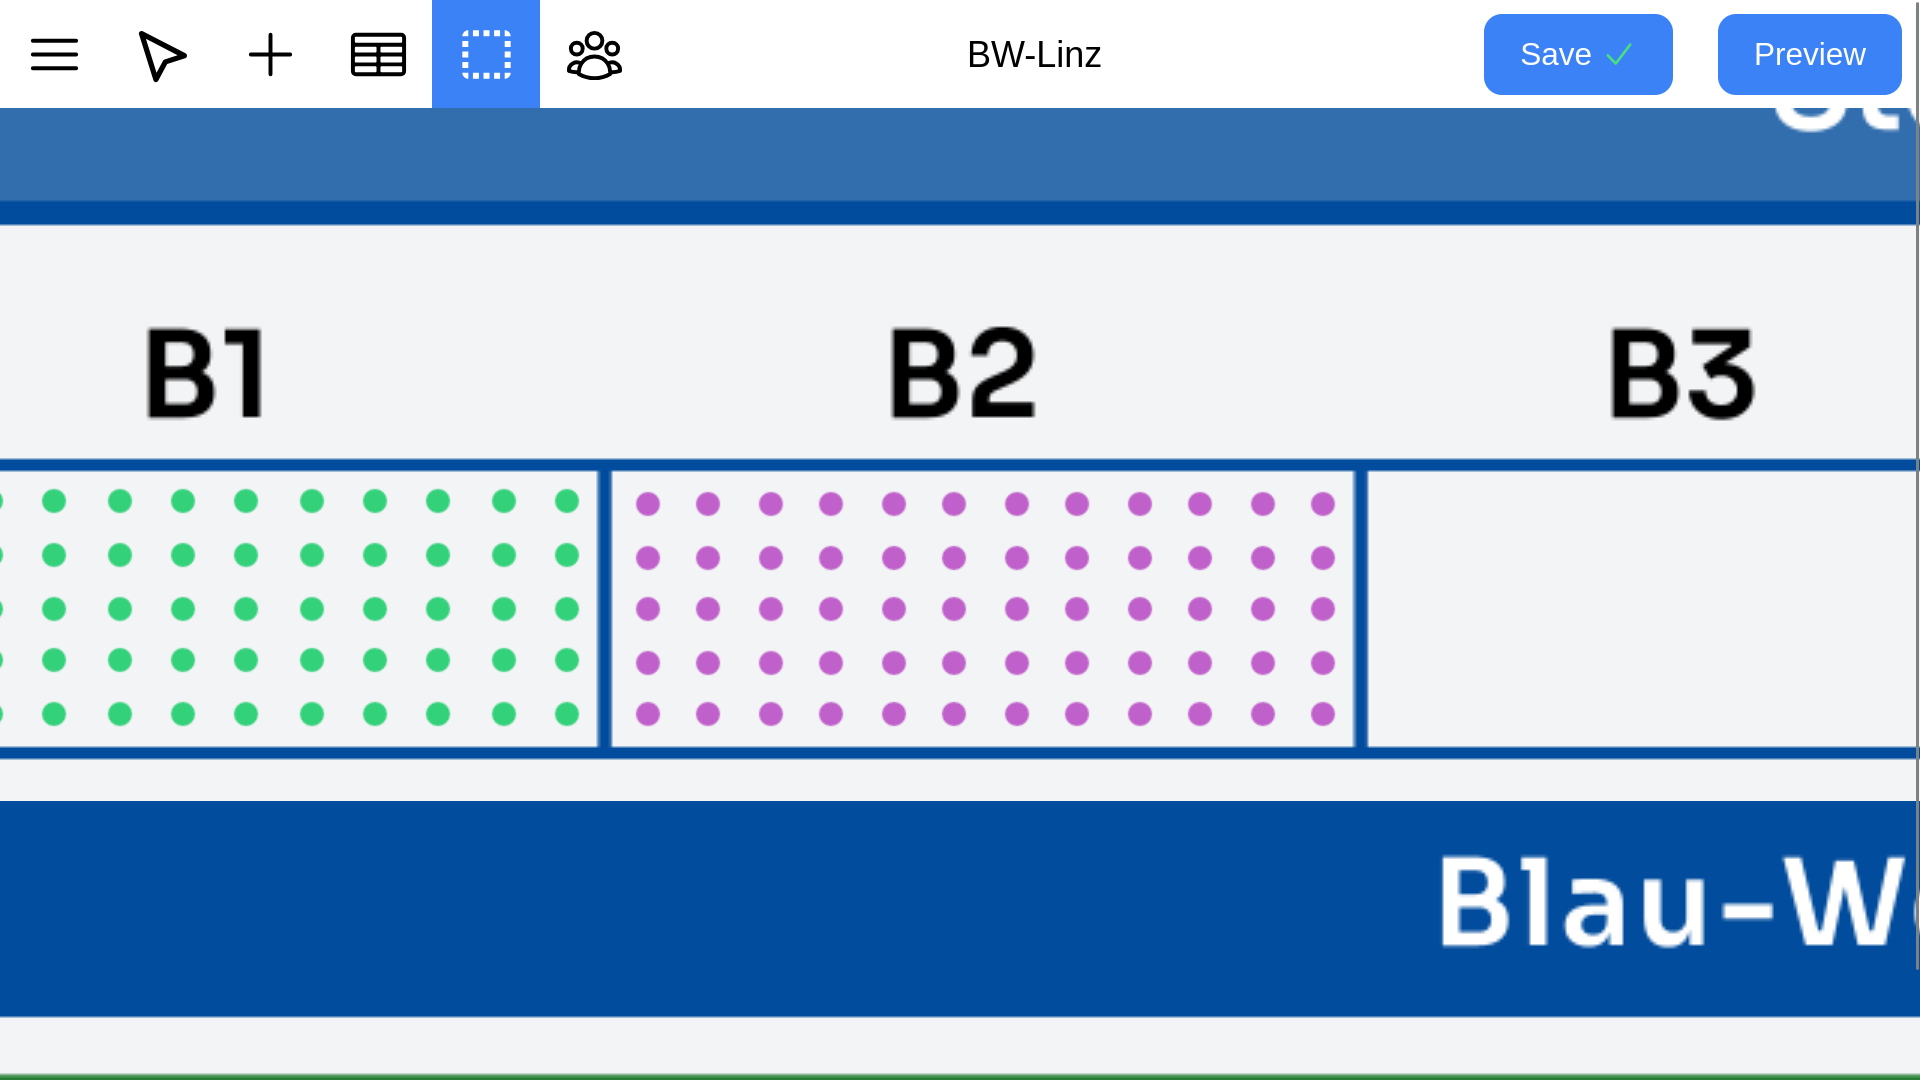
\includegraphics[width=0.4\textwidth]{pics/abstract.png}
    \end{center}
\end{wrapfigure}
SeatGen ist ein Tool, das für die Solvistas GmbH entwickelt wurde, um die Erstellung und Verwaltung von Stadion-Sitzplänen zu vereinfachen. Es ersetzt den bisher ineffizienten manuellen Prozess durch eine intuitive grafische Benutzeroberfläche und ermöglicht es Veranstaltern, Sitzpläne ohne technisches Vorwissen zu entwerfen und zu bearbeiten.

Die Anwendung wurde mit React, Spring Boot \& Kotlin sowie Leaflet.js umgesetzt und erlaubt die direkte Bearbeitung von Sitzplätzen, Echtzeit-Aktualisierungen sowie Massenbearbeitungen. Diese Arbeit beleuchtet die Herausforderungen, eingesetzten Technologien und die Umsetzung von SeatGen.
\newpage
